\documentclass[12pt,onecolumn]{article}
\usepackage[utf8]{inputenc} % UTF8 input encoding
\usepackage[T2A]{fontenc}   % T2A font encoding for Cyrillic script
\usepackage[russian]{babel} % Russian language support
\usepackage{listings}
\usepackage{float}
\usepackage{mathtools}
\usepackage{longtable}
\usepackage{multicol}
\usepackage{lipsum}
\everymath{\displaystyle}
\usepackage{listings} 
\usepackage[usenames]{color}
\usepackage{geometry}
\geometry{
  a4paper,
  top=25mm, 
  right=15mm, 
  bottom=25mm, 
  left=15mm
}

\begin{document}
\setcounter{tocdepth}{4}
\begin{center}
    Федеральное государственное автономное образовательное учреждение высшего образования "Национальный Исследовательский Университет ИТМО"\\ 
    Мегафакультет Компьютерных Технологий и Управления\\
    Факультет Программной Инженерии и Компьютерной Техники \\
    
\includegraphics[scale=0.3]{image/itmo.jpg} % нужно закинуть картинку логтипа в папку с отчетом
\end{center}
\vspace{1cm}


\begin{center}
    \textbf{Лабораторная работа №2}\\
    по дисциплине\\
    \textbf{'Информационные системы и базы данных'}\\
    \textbf{Вариант 3893 / 3NF}
\end{center}

\vspace{2cm}

\begin{flushright}
  Выполнил Студент  группы P32101\\
  \textbf{Лапин Алексей Александрович}\\
  Преподаватель: \\
  \textbf{Сагайдак Алина Алексеевна}\\
\end{flushright}

\vspace{6cm}
\begin{center}
    г. Санкт-Петербург\\
    2023г.
\end{center}

\newpage
\tableofcontents
\newpage

\section{Текст задания.}
Для отношений, полученных при построении предметной области из
лабораторной работы №1, выполните следующие действия:
\begin{enumerate}
  \item Опишите функциональные зависимости для отношений полученной схемы (минимальное множество);
  \item Приведите отношения в 3NF (как минимум). Постройте схему на основеNF (как минимум). Постройте схему на основе
  полученных отношений;
  \item Опишите изменения в функциональных зависимостях, произошедшие после преобразования в 3NF (как минимум). Постройте схему на основеNF;
  \item Какие денормализации будут полезны для вашей схемы? Приведите
  подробное описание;
\end{enumerate}
\section{Описание предметной области.}
Он не стал дожидаться ответа и правильно сделал. Сирэйнис даже не пошевельнулась, но он тотчас же почувствовал, что его тело перестает ему повиноваться. Сила, столкнувшаяся с его волей, оказалась куда более могущественной, чем он ожидал, и это навело его на мысль, что Сирэйнис, возможно, помогало огромное число людей. Беспомощно повлекся он обратно к дому, и на какой-то ужасный момент ему даже подумалось, что великолепный его план провалился.\\
\textbf{Творческий пересказ:}\\
Люди хотят достичь некоторых целей. Для достижения целей, люди строят планы, которые состоят из определенного набора шагов разной сложности. Чтобы преодолеть сложности на своём пути люди обладают силой воли и поддержкой других людей. Так же у людей есть свой дом или несколько домов, где они живут с другими жильцами, которые могут быть им родственниками , друзьями, а порой даже врагами. 
\section{Даталогическая модель}
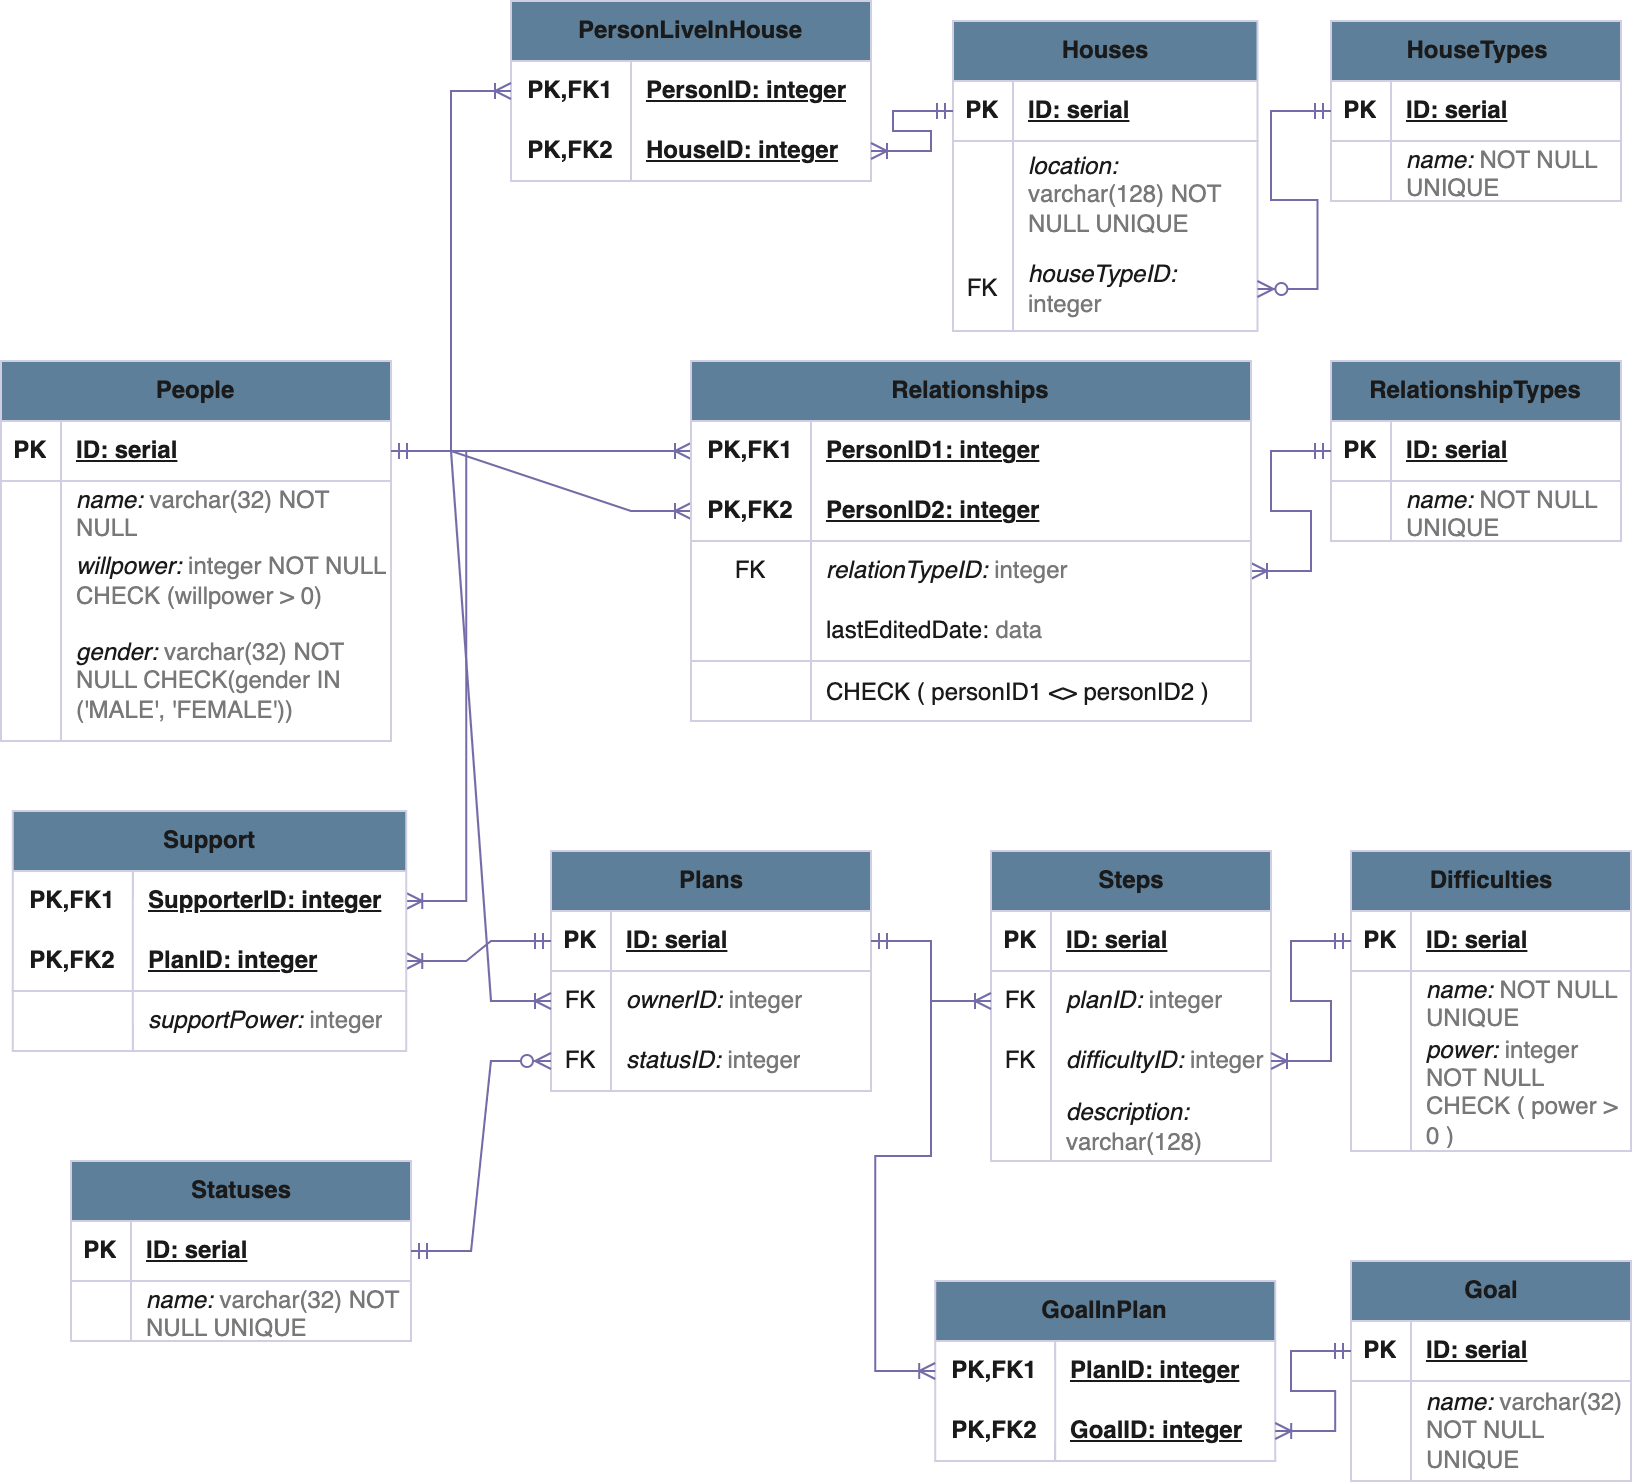
\includegraphics[width=\textwidth]{image/datalogical-model.png}
\newpage
\section{Опишите функциональные зависимости для отношений полученной схемы (минимальное множество);}
\begin{multicols}{2}
  \textbf{People}\\
  id $\to$ name\\
  id $\to$ willpower\\
  id $\to$ gender\\
  \textbf{Houses}\\
  id $\to$ location\\
  id $\to$ houseTypeID\\
  location $\to$ houseTypeID\\
  \textbf{HouseTypes}\\
  id $\to$ name\\
  \textbf{Relationships}\\
  PersonID1, PersonID2 $\to$ relationshipTypeID\\
  PersonID1, PersonID2 $\to$ lastEditedDate\\
  \textbf{RelationshipTypes}\\
  id $\to$ name\\
  \textbf{Support}\\
  SupporterID, PlanID $\to$ supportPower\\
  \textbf{Statuses}\\
  id $\to$ name\\
  \textbf{Plans}\\
  id $\to$ ownerID\\
  id $\to$ statusID\\
  \textbf{Steps}\\
  id $\to$ planID\\
  id $\to$ difficultyID\\
  id $\to$ description\\
  \textbf{Difficulties}\\
  id $\to$ name\\
  id $\to$ power\\
  name $\to$ power\\
  \textbf{Goal}\\
  id $\to$ name\\
\end{multicols}
\section{Приведите отношения в 3NF (как минимум). Постройте схему на основе 3NF (как минимум). Постройте схему на основе
полученных отношений;}
\textbf{1NF:} Отношение, на пересечении каждой строки и столбца одно значение.\\
Все мои таблицы удовлетворяют этому условию.\\
\textbf{2NF:} Отношение находится в 1НФ и каждый его атрибут полностью зависит от первичного ключа.\\
Чтобы привести к 2НФ — убрать частичные зависимости от ключа:
\begin{itemize}
  \item удалить атрибуты, зависящие от составляющих ключа из $R_1$;
  \item новое отношение $R_2$: удаленные атрибуты из $R_1$ + соответствующий детерминант;
\end{itemize}
Все таблицы удовлетворяют условиям 2НФ. Следовательно в данном случае преобразования не требуются.\\
\textbf{3NF:} отношение в 1) 1НФ и 2НФ и 2) все атрибуты, которые не входят в первичный ключ, не находятся в транзитивной функциональной зависимости от первичного ключа.\\
Чтобы привести к 3НФ — убрать транзитивные зависимости:
\begin{itemize}
  \item удалить из $R_1$ атрибуты, транзитивно-зависимые от первичного ключа;
  \item новое отношение $R_2$: атрибуты (удаленные в 1.) + соответствующий детерминант;
\end{itemize}
Таблица Difficulties не удовлетворяет условиям 3НФ, так как некоторые её атрибуты транзитивно зависят от первичного ключа: id $\to$ name $\to$ power.\\
Следовательно, для того чтобы привести таблицу Difficulties к 3НФ, необходимо разбить её на две таблицы:\\
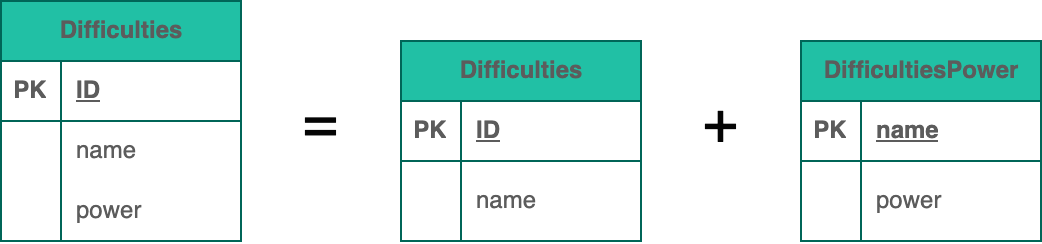
\includegraphics[width=\textwidth]{image/lab2.png}
\section{Опишите изменения в функциональных зависимостях, произошедшие
после преобразования в 3NF (как минимум)}
\begin{multicols}{2}

  \noindent\underline{Было:}\\
  \textbf{Difficulties}\\
  id $\to$ name\\
  id $\to$ power\\
  name $\to$ power\\
  \mbox{}\\
  \underline{Стало:}\\
  \textbf{Difficulties}\\
  id $\to$ name\\
  \textbf{DifficultiesPower}\\
  name $\to$ power\\
\end{multicols}
\section{Какие денормализации будут полезны для вашей схемы? Приведите
подробное описание}

Я думаю, что декомпозиция таблицы Difficulties была лишней, так как получившиеся таблицы Difficulties и
DifficultiesPower являются слишком маленькими и не имеют смысла по отдельности, так как id добавлялся в Difficulties, для того чтобы не писать возможно длинные имена сложностей и поддерживать возможность быстрой смены имени без смены ID и power (например 'done' на 'finished'). Также эффективность запросов из-за уменьшения числа соединений должна повысится. А плюсы нормализации в данном случае не столь очевидны.\\

\section{Вывод}
В ходе выполнения лабораторной работы №2 были изучены функциональные зависимости, нормализация и денормализация баз данных. Были получены навыки работы с нормализацией и денормализацией баз данных.
\end{document}